\documentclass[11pt,border=2pt]{standalone}
\usepackage{amsmath,amssymb}
\usepackage{xcolor}
\usepackage{tikz}
\usepackage{pgfplots}
\pgfplotsset{compat=1.18}
\usetikzlibrary{calc,arrows,positioning,fit,backgrounds,decorations.pathreplacing,patterns}
\definecolor{cElem}{RGB}{40,80,140}
\definecolor{cTrg}{RGB}{190,40,40}
\definecolor{cCell}{RGB}{225,238,248}
\definecolor{cAcc}{RGB}{240,200,120}
\definecolor{cGrey}{RGB}{120,120,120}
\definecolor{cVec}{RGB}{110,55,150}
\begin{document}
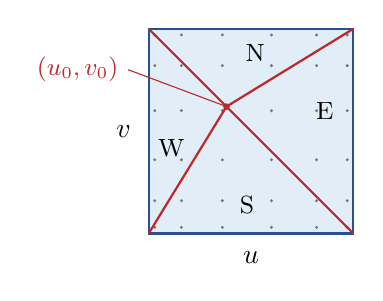
\begin{tikzpicture}[scale=2.6]
  \def\ux{0.38} \def\vy{0.62}
  \fill[cCell] (0,0) rectangle (1,1);
  \draw[cElem,thick] (0,0) rectangle (1,1);
  % GL-ish nodes
  \foreach \x in {0.03,0.16,0.36,0.60,0.82,0.97}
    \foreach \y in {0.03,0.16,0.36,0.60,0.82,0.97}
      \fill[cGrey] (\x,\y) circle (0.008);
  % the four triangles
  \draw[cTrg,thick] (\ux,\vy) -- (0,0);
  \draw[cTrg,thick] (\ux,\vy) -- (1,0);
  \draw[cTrg,thick] (\ux,\vy) -- (1,1);
  \draw[cTrg,thick] (\ux,\vy) -- (0,1);
  \fill[cTrg] (\ux,\vy) circle (0.016);
  \draw[cTrg,thin] (\ux,\vy) -- (-0.10,0.80);
  \node[cTrg,font=\small,left=0pt] at (-0.10,0.80) {$(u_0,v_0)$};
  \node[font=\small] at (0.48,0.14) {S};
  \node[font=\small] at (0.86,0.60) {E};
  \node[font=\small] at (0.52,0.88) {N};
  \node[font=\small] at (0.11,0.42) {W};
  \node[below] at (0.5,-0.04) {$u$};
  \node[left]  at (-0.04,0.5) {$v$};
\end{tikzpicture}
\end{document}
